\begin{figure}[!htbp]
\centering
\begin{minipage}[t]{.485\linewidth}
\centering
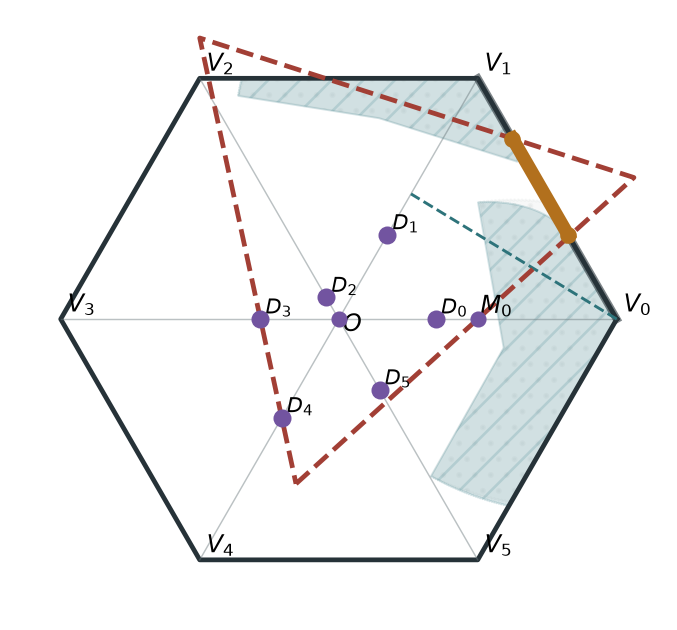
\includegraphics[width=\linewidth]
  {figures/trace_exact_ab/one_gap_n1_t3.png}
\par\smallskip
\textbf{One gap.}\par\smallskip
{\footnotesize
\(\begin{gathered}
N_{\rm gap}=1\\
N_+=1\\
(d,t)=(0,1)
\end{gathered}\)}
\end{minipage}\hfill
\begin{minipage}[t]{.485\linewidth}
\centering
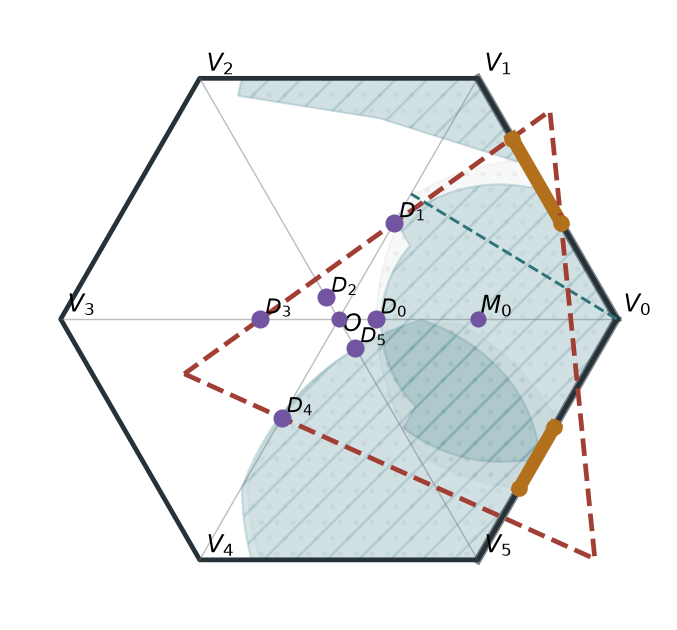
\includegraphics[width=\linewidth]
  {figures/trace_exact_ab/two_gap_n1_t3.png}
\par\smallskip
\textbf{Two gaps.}\par\smallskip
{\footnotesize
\(\begin{gathered}
N_{\rm gap}=2\\
N_+=1\\
(d,t)=(0,1)
\end{gathered}\)}
\end{minipage}
\caption{Case \(D_T\): sampled \(\Tlike\) supported-tail data.}
\label{fig:finite-enclosure-case-dt-examples}
\end{figure}
